
\subsection{Answers}
\begin{table}[htb]%
\begin{center}%
\caption{Q27: What MPI feature(s) are NOT useful for you application?}%
\label{tab:Q27-ans}%
\begin{tabular}{l|l|r}%
\hline%
Choice & Abbrv. & \# Answers \\%
\hline%
There are no unnecessary features & No & 309 (41.5\%) \\%
Dynamic process creation & Dyn. process & 274 (36.8\%) \\%
Process topologies & Topologies & 126 (16.9\%) \\%
One-sided communication & One-sided & 103 (13.8\%) \\%
Error handlers & Error & 72 (9.7\%) \\%
Communicator and group management & Communicator & 63 (8.5\%) \\%
Datatypes & Datatypes & 58 (7.8\%) \\%
Collective operations & Collectives & 11 (1.5\%) \\%
other & - & 20 (2.7\%) \\%
\hline%
\multicolumn{2}{c}{total} & 1036 (745)\\%
\hline%
\end{tabular}%
\end{center}%
\end{table}%

\clearpage%
{\footnotesize\begin{landscape}%
\begin{longtable}[htb]{r|c|c|c|c|c|c|c|c|c|c}%
\caption{Q27: What MPI feature(s) are NOT useful for you application?}%
\label{tab:Q27-mans} \\%
\hline%
Multi-Answer & overall & FR & GR & IT & UK & eu & JP & RU & US & others \\
 \hline%
\endfirsthead%
\multicolumn{11}{r}{(continued from the previous page)}\\%
\hline%
Multi-Answer & overall & FR & GR & IT & UK & eu & JP & RU & US & others \\
 \hline%
\endhead%
\hline%
(total) & 745 & 106 & 136 & 51 & 61 & 123 & 61 & 85 & 49 & 73 \\%
\hline%
\multicolumn{11}{r}{(continue to the next page)}\\%
\endfoot%
\hline%
(total) & 745 & 106 & 136 & 51 & 61 & 123 & 61 & 85 & 49 & 73 \\%
\hline%
\endlastfoot%
\hline%
{No unnecessary feature} & 307 & 34 & 56 & 26 & 30 & 49 & 19 & 34 & 16 & 43 \\%
{Dynamic process} & 120 & 15 & 20 & 9 & 12 & 20 & 9 & 16 & 11 & 8 \\%
{Topologies, Dynamic process} & 33 & 8 & 6 & 2 & 3 & 6 & 1 & 2 & 3 & 2 \\%
{One-sided} & 30 & 5 & 8 & 0 & 1 & 3 & 4 & 4 & 1 & 4 \\%
{One-sided, Dynamic process} & 25 & 4 & 4 & 1 & 3 & 6 & 2 & 3 & 2 & 0 \\%
{Topologies} & 21 & 3 & 2 & 3 & 1 & 5 & 1 & 2 & 1 & 3 \\%
{Dynamic process, Error} & 18 & 1 & 6 & 0 & 0 & 4 & 2 & 1 & 2 & 2 \\%
{Datatypes} & 18 & 6 & 1 & 0 & 0 & 6 & 3 & 1 & 1 & 0 \\%
{Error} & 17 & 1 & 2 & 2 & 0 & 2 & 3 & 0 & 3 & 4 \\%
{Communicator} & 16 & 3 & 3 & 3 & 0 & 1 & 3 & 1 & 1 & 1 \\%
{Datatypes, Dynamic process} & 11 & 3 & 1 & 1 & 2 & 1 & 2 & 0 & 1 & 0 \\%
{One-sided, Topologies, Dynamic process} & 9 & 3 & 0 & 0 & 2 & 3 & 0 & 1 & 0 & 0 \\%
{Communicator, Topologies, Dynamic process} & 8 & 0 & 0 & 0 & 2 & 0 & 2 & 4 & 0 & 0 \\%
{One-sided, Topologies} & 7 & 2 & 2 & 0 & 1 & 1 & 0 & 1 & 0 & 0 \\%
{Communicator, Dynamic process} & 7 & 2 & 1 & 1 & 1 & 0 & 1 & 1 & 0 & 0 \\%
{Topologies, Dynamic process, Error} & 7 & 0 & 1 & 0 & 1 & 4 & 0 & 0 & 1 & 0 \\%
{One-sided, Topologies, Dynamic process, Error} & 7 & 3 & 2 & 0 & 0 & 1 & 0 & 1 & 0 & 0 \\%
{Datatypes, Topologies} & 6 & 0 & 1 & 0 & 0 & 1 & 0 & 2 & 1 & 1 \\%
{Datatypes, Communicator} & 5 & 0 & 1 & 2 & 0 & 0 & 0 & 2 & 0 & 0 \\%
{Communicator, Topologies, Dynamic process, Error} & 4 & 1 & 0 & 0 & 1 & 0 & 1 & 1 & 0 & 0 \\%
{Communicator, Topologies} & 4 & 0 & 1 & 0 & 0 & 1 & 1 & 0 & 0 & 1 \\%
{Collectives} & 4 & 0 & 0 & 0 & 0 & 1 & 0 & 1 & 1 & 1 \\%
{One-sided, Communicator, Dynamic process} & 4 & 2 & 2 & 0 & 0 & 0 & 0 & 0 & 0 & 0 \\%
{One-sided, Communicator, Topologies, Dynamic process, Error} & 3 & 0 & 2 & 0 & 0 & 0 & 0 & 1 & 0 & 0 \\%
{Topologies, Error} & 3 & 0 & 1 & 0 & 0 & 0 & 2 & 0 & 0 & 0 \\%
{One-sided, Datatypes} & 3 & 2 & 1 & 0 & 0 & 0 & 0 & 0 & 0 & 0 \\%
{One-sided, Dynamic process, Error} & 3 & 1 & 1 & 0 & 0 & 0 & 0 & 1 & 0 & 0 \\%
{One-sided, Communicator} & 2 & 1 & 1 & 0 & 0 & 0 & 0 & 0 & 0 & 0 \\%
{Datatypes, Topologies, Dynamic process} & 2 & 1 & 1 & 0 & 0 & 0 & 0 & 0 & 0 & 0 \\%
{One-sided, Communicator, Topologies, Dynamic process} & 2 & 0 & 0 & 1 & 1 & 0 & 0 & 0 & 0 & 0 \\%
{Datatypes, Dynamic process, Error} & 2 & 0 & 1 & 0 & 0 & 0 & 1 & 0 & 0 & 0 \\%
{One-sided, Datatypes, Communicator, Collectives} & 2 & 0 & 0 & 0 & 0 & 1 & 0 & 1 & 0 & 0 \\%
{I'm not sure} & 1 & 0 & 0 & 0 & 0 & 0 & 0 & 1 & 0 & 0 \\%
{Datatypes, Communicator, Collectives} & 1 & 0 & 0 & 0 & 0 & 0 & 1 & 0 & 0 & 0 \\%
{Error, Tag matching is not needed most of the time. I would exchange it in return for more performance.} & 1 & 0 & 0 & 0 & 0 & 0 & 0 & 0 & 0 & 1 \\%
{Topologies, Dynamic process, I/O} & 1 & 0 & 0 & 0 & 0 & 0 & 0 & 0 & 1 & 0 \\%
{One-sided, Error} & 1 & 1 & 0 & 0 & 0 & 0 & 0 & 0 & 0 & 0 \\%
{Communicator, Collectives, Topologies, Dynamic process} & 1 & 0 & 0 & 0 & 0 & 1 & 0 & 0 & 0 & 0 \\%
{all of the above are useful} & 1 & 0 & 0 & 0 & 0 & 0 & 0 & 0 & 1 & 0 \\%
{One-sided, Datatypes, Communicator, Collectives, Topologies, Dynamic process, Error} & 1 & 0 & 0 & 0 & 0 & 1 & 0 & 0 & 0 & 0 \\%
{no clue} & 1 & 0 & 0 & 0 & 0 & 1 & 0 & 0 & 0 & 0 \\%
{One-sided, Datatypes, Topologies, Dynamic process, Error} & 1 & 0 & 0 & 0 & 0 & 0 & 0 & 0 & 1 & 0 \\%
{I use only a small part of the MPI features} & 1 & 0 & 1 & 0 & 0 & 0 & 0 & 0 & 0 & 0 \\%
{Topologies, Error, No unnecessary feature} & 1 & 0 & 0 & 0 & 0 & 0 & 0 & 0 & 0 & 1 \\%
{I am not sure because I don't have the full overview} & 1 & 0 & 1 & 0 & 0 & 0 & 0 & 0 & 0 & 0 \\%
{Datatypes, Topologies, Dynamic process, Error} & 1 & 0 & 0 & 0 & 0 & 0 & 0 & 1 & 0 & 0 \\%
{Collectives, Topologies} & 1 & 0 & 0 & 0 & 0 & 0 & 0 & 0 & 0 & 1 \\%
{do not know} & 1 & 0 & 1 & 0 & 0 & 0 & 0 & 0 & 0 & 0 \\%
{Datatypes, Communicator, Dynamic process} & 1 & 0 & 0 & 0 & 0 & 0 & 0 & 1 & 0 & 0 \\%
{Datatypes, Communicator, Topologies, Dynamic process} & 1 & 0 & 0 & 0 & 0 & 0 & 0 & 0 & 1 & 0 \\%
{I don't know} & 1 & 0 & 1 & 0 & 0 & 0 & 0 & 0 & 0 & 0 \\%
{I don't know.} & 1 & 0 & 0 & 0 & 0 & 0 & 1 & 0 & 0 & 0 \\%
{One-sided, Datatypes, Dynamic process} & 1 & 1 & 0 & 0 & 0 & 0 & 0 & 0 & 0 & 0 \\%
{Topologies, I don't think I need them. But they are useful for domain decomposition.} & 1 & 0 & 0 & 0 & 0 & 1 & 0 & 0 & 0 & 0 \\%
{I am not sure} & 1 & 0 & 0 & 0 & 0 & 0 & 1 & 0 & 0 & 0 \\%
{I am not aware of unncessary features, but maybe my overview is not large enough.} & 1 & 0 & 1 & 0 & 0 & 0 & 0 & 0 & 0 & 0 \\%
{things I don't know like Dynamic process creation etc} & 1 & 1 & 0 & 0 & 0 & 0 & 0 & 0 & 0 & 0 \\%
{the performance of some features needs improvement} & 1 & 0 & 1 & 0 & 0 & 0 & 0 & 0 & 0 & 0 \\%
{Communicator, Collectives} & 1 & 1 & 0 & 0 & 0 & 0 & 0 & 0 & 0 & 0 \\%
{One-sided, Datatypes, Dynamic process, Error} & 1 & 1 & 0 & 0 & 0 & 0 & 0 & 0 & 0 & 0 \\%
{Don't know (too little experience with MPI)} & 1 & 0 & 0 & 0 & 0 & 0 & 0 & 1 & 0 & 0 \\%
{Haven't tried all. So can not comment} & 1 & 0 & 1 & 0 & 0 & 0 & 0 & 0 & 0 & 0 \\%
{One-sided, Datatypes, Error} & 1 & 0 & 0 & 0 & 0 & 0 & 1 & 0 & 0 & 0 \\%
{I do not know :)} & 1 & 0 & 0 & 0 & 0 & 1 & 0 & 0 & 0 & 0 \\%
{Don't know} & 1 & 0 & 1 & 0 & 0 & 0 & 0 & 0 & 0 & 0 \\%
{Topologies, No unnecessary feature} & 1 & 0 & 0 & 0 & 0 & 1 & 0 & 0 & 0 & 0 \\%
{I do not know} & 1 & 0 & 0 & 0 & 0 & 1 & 0 & 0 & 0 & 0 \\%
\hline%
\end{longtable}%
\end{landscape}}%
\clearpage%


This question tries to look at the standard from the opposite point of view,
asking not about the missing parts but about the unnecessary features for the
user’s applications related on the perceived usefulness of each chapter of the
MPI standards for users applications. Unsurprisingly, the least unwanted feature
is the collective operation: this feature is seen as very important and very
useful. Datatypes, communicators and group management as well as  error handlers
received less than 10\% of the answers and are therefore seen as very useful
characteristics of the standard. On the other side, dynamic process creation
received 29\% of the answers. This means that such feature is not used in many
applications and that more generally, MPI is seen as a static programming model
where the number of processes does not evolve during the program execution. To a
least extent, process topologies and one-sided communication received
respectively 12\% and 10\% of the answers. This is not very surprising as these
features relatively specific to special use-cases.

The usefulness of dynamic processing can be regarded from different
perspectives. Without delving into MPI implementation details or HPC center
administration, dynamic processing was certainly always the least, and possibly
the last, supported capability in MPI. This is not a new trend, it was
consistent starting from the moment when this feature was accepted into the MPI
standard. We might be facing a chicken and egg problem, a feature being unused,
or mostly unknown to users due to it's lack of support, or, the opposite, the
lack of support due to user lack of interest. In any case, several recent
studies pinpoint to the need for such feature outside the HPC market.

\todo{It is a bit odd that the most people say the collective ops is useful,
however, 61 people feel that communicators (and group) ops are useless. Does
this mean many MPI users do not create their own communicators?}

\subsection{List of other answers}
\begin{itemize}
\item Europe:France: things I don't know like Dynamic process creation etc
\item Europe:Germany: Don't know
\item Europe:Germany: Haven't tried all. So can not comment
\item Europe:Germany: I am not aware of unncessary features, but maybe my overview is not large enough.
\item Europe:Germany: I am not sure because I don't have the full overview
\item Europe:Germany: I don't know
\item Europe:Germany: I use only a small part of the MPI features
\item Europe:Germany: do not know
\item Europe:Germany: the performance of some features needs improvement
\item Europe:others: I do not know
\item Europe:others: I do not know :)
\item Europe:others: I don't think I need them. But they are useful for domain decomposition.
\item Europe:others: no clue
\item Japan: I am not sure
\item Japan: I don't know.
\item North America: Tag matching is not needed most of the time. I would exchange it in return for more performance.
\item Russia: Don't know (too little experience with MPI)
\item Russia: I'm not sure
\item USA: I/O
\item USA: all of the above are useful

\end{itemize}

\begin{figure}[htb]
\begin{center}
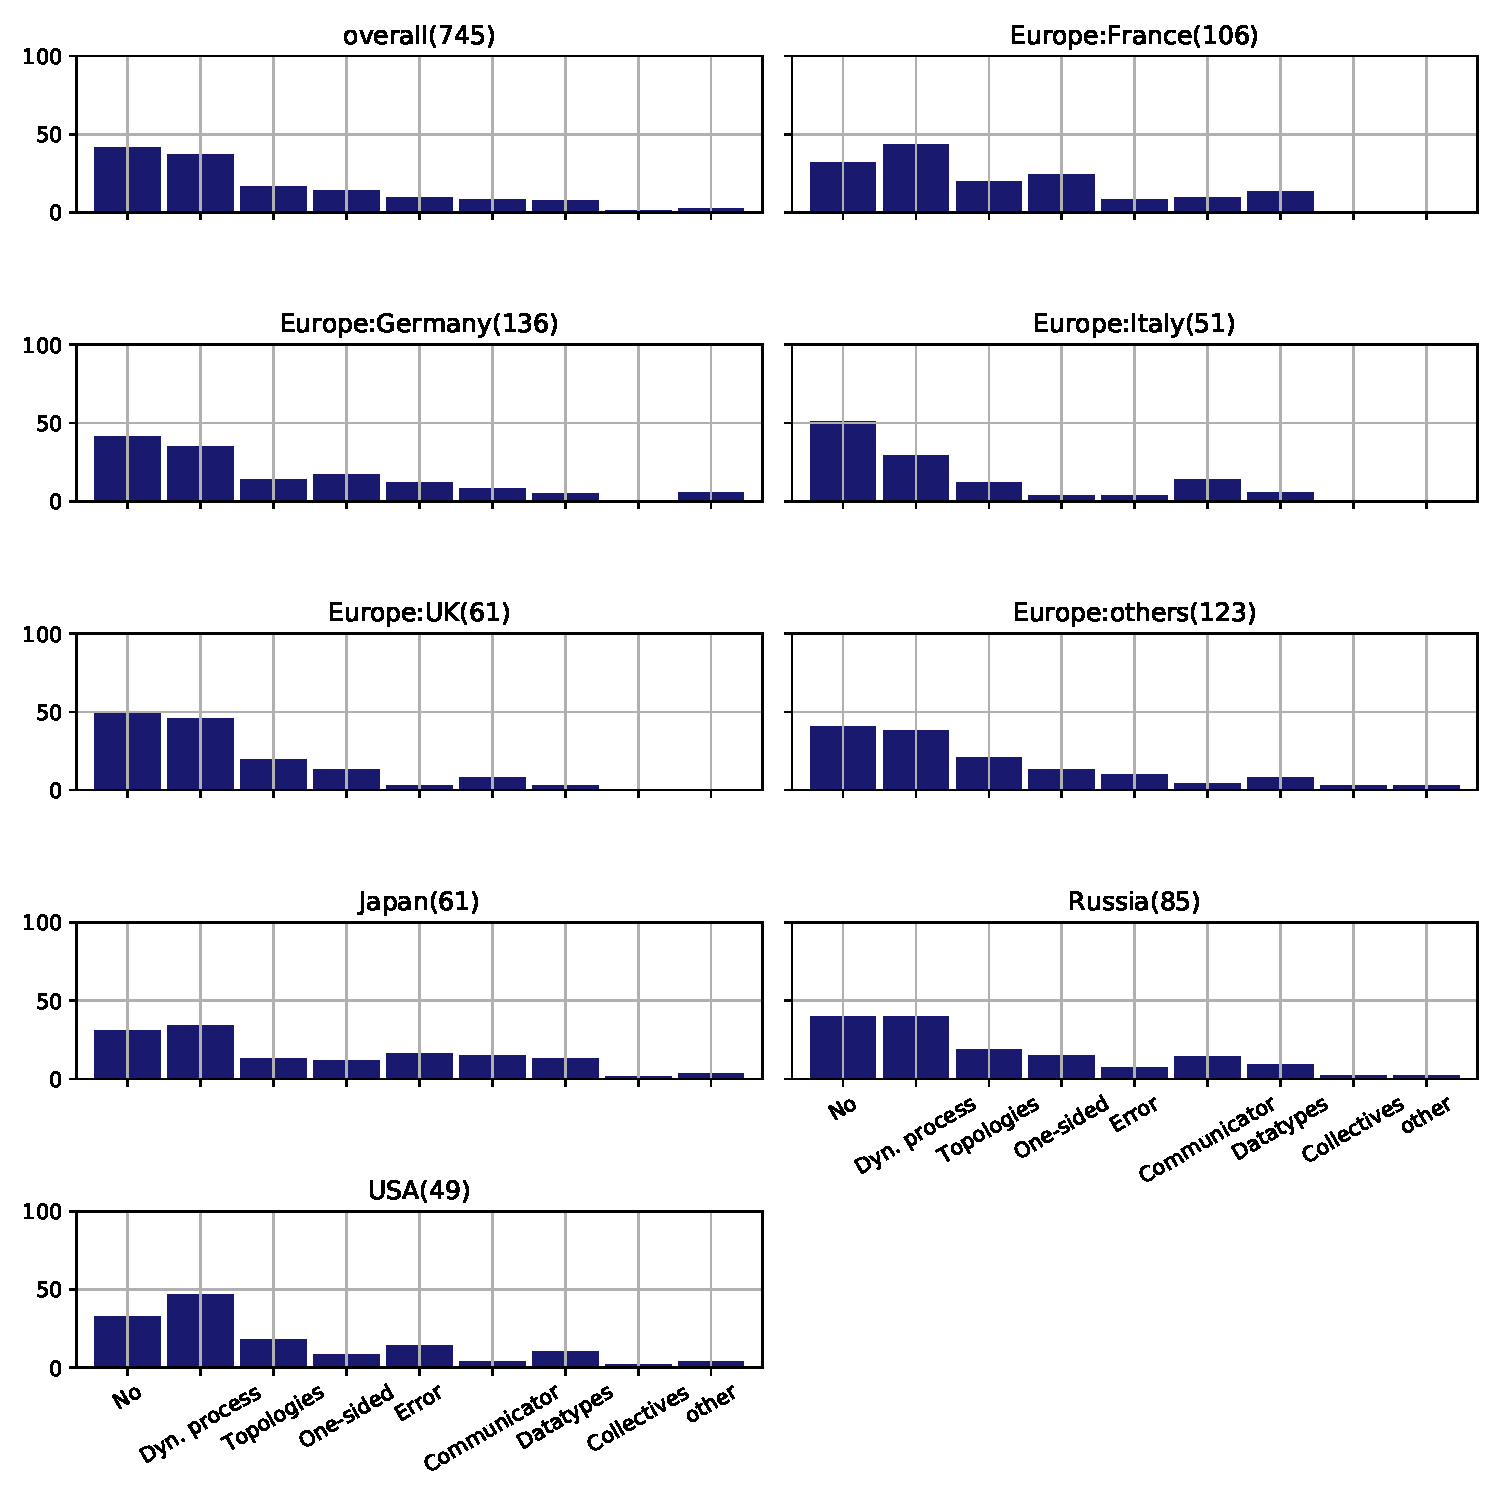
\includegraphics[width=10cm]{../pdfs/Q27.pdf}
\caption{Simple analysis: Q27}
\label{fig:Q27}
\end{center}
\end{figure}

\begin{figure}[htb]
\begin{center}
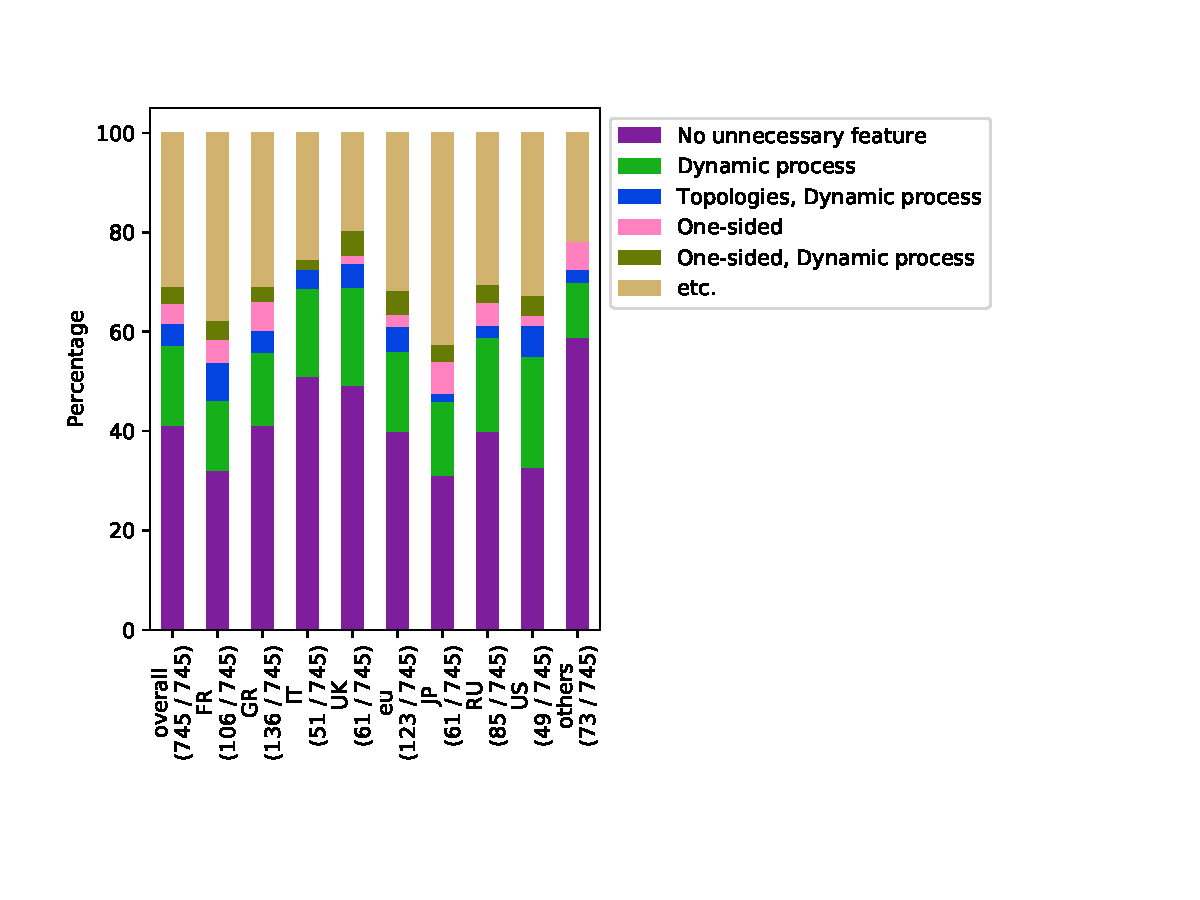
\includegraphics[width=14cm]{../pdfs/Q27-mans.pdf}
\caption{Multiple Answers: Q27}
\label{fig:Q27-mans}
\end{center}
\end{figure}
